%  ----------------------------------------------------------------------------
% Dieses Dokument ist eine Kurzversion von:
%
% Copyright (c) 2016 by Burkhardt Renz. All rights reserved.
% Vorlage Abschlussarbeit THM (minimal)
% $Id: vorlage.tex 3811 2016-08-05 12:03:51Z br $
% 
% Der Dokumentstyle wurde von "srcbook" auf "article" geändert, 
% um den Einstieg in LaTex zu erleichtern. 
% Die Unterdateien wurden nicht per \input ins Dokument geholt, 
% sondern direkt eingefügt. Chapters wurden in Sections 
% umbenannt. Das Titelblatt wurde verändert.
% Die Beschreibung der labeling-Umgebung wurde entfernt. ----------------------------------------------------------------------------

\documentclass[11pt]{scrartcl}       % KOMA-Skript für Artikel
\RequirePackage{filecontents}
\usepackage{color,soul}
%% Präambel
\usepackage[english, ngerman]{babel} % deutsche typogr. Regeln + Trenntabelle
\usepackage[T1]{fontenc}             % interner TeX-Font-Codierung
\usepackage{lmodern}                 % Font Latin Modern
\usepackage[utf8]{inputenc}          % Font-Codierung der Eingabedatei
\usepackage[babel]{csquotes}         % Anführungszeichen
\usepackage{graphicx}                % Graphiken
\usepackage{booktabs}                % Tabellen schöner
\usepackage{listingsutf8}            % Listings mit Einstellungen
\usepackage[
backend=biber,			% Biber Compiler
style=alphabetic,  		% alphanumeric Labels
sorting=anyt 			% sort by alphabetic label, name, year, title 
]{biblatex}				% BibLaTex
\addbibresource{References.bib}

\lstset{basicstyle=\small\ttfamily,
	tabsize=2,
	basewidth={0.5em,0.45em},
	extendedchars=true}
\usepackage{amsmath}	               % Mathematik
\usepackage[pdftex]{hyperref}       
\hypersetup{
	bookmarksopen=true,
	bookmarksopenlevel=3,
	colorlinks,
	citecolor=blue,
	linkcolor=blue,
}
\usepackage{scrhack}								 % unterdrückt Fehlermeldung von listings

%% Nummerierungstiefen
\setcounter{tocdepth}{3}             % 3 Stufen im Inhaltsverzeichnis
\setcounter{secnumdepth}{3} 		 % 3 Stufen in Abschnittnummerierung

% ----------------------------------------------------------------------------
\begin{document}



%% Titelseite
	
\titlehead{

\includegraphics[width=0.9\textwidth]{img/mni-logo}
}
\title{Einige wesentliche Kriterien für die Auswahl von Software für ein QMS}
\author{Assem Hussein}
\date{Winter 2021/2022}
\maketitle	


\newpage
%% Verzeichnissse
 \tableofcontents
%% \listoffigures
%% \listoftables
%\lstlistoflistings

\newpage

\section{Einleitung}
Die Auswahl eines wirksamen QMS\footnote{QMS wird näher definiert in Paragraph 3.1 } ist eine nicht triviale Herausforderung, die einen besonderen Ansatz erfordert. Immer mehr Organisationen streben täglich danach, ein QMS einzuführen und sich zertifizieren zu lassen. Heute übersteigt die Zahl der zertifizierten QMS 1,5 Millionen \cite{Leontyuk_2019}. Ein solch gravierender Trend muss sich bei der Erfüllung der gesetzlichen Anforderungen als wirksam erwiesen haben und gleichzeitig die Kundenzufriedenheit erhöhen, was wiederum zu höheren Gewinnen führt.
\\
\\
Hierbei werden allgemeine Verfahren für die Softwareauswahl vorgestellt und die Hauptkriterien der Softwareauswahl erläutert. Insbesondere werden die wesentlichen Kriterien für die Auswahl eines QMS im Detail betrachtet.


\section{Allgemeines Verfahren für die Softwareauswahl}

TODO


\subsection{Gängige Ansätze}

TODO


\subsection{Allgemeine Kriterien}

TODO

 

\subsubsection{Kriterium/Kategorie A}

TODO


\subsubsection{Kriterium/Kategorie B}

TODO


\subsubsection{Kriterium/Kategorie C}

TODO


\subsubsection{Kriterium/Kategorie D}

TODO

\newpage
\section{Was ist ein QMS?}
\subsection{Definition und Anwendungsgebiet}
Ein Qualitätsmanagementsystem (kurz: QMS) ist eine Methode der Unternehmensführung, die als Werkzeug zur Qualitätssicherung dient. Ziel ist ein systematisches Qualitätsmanagement durch klare Zielsetzung und effizientes Steuern von Prozessen und Ressourcen. Das soll sicherstellen, dass die Interessen aller beteiligten Parteien (vor allem Kunden) verwirklicht werden. Auf ähnliche Weise erläutert \citeauthor{mai2020grundlage} in \citeyear{mai2020grundlage}, was ein QMS ist:

\begin{quotation}
„Der Begriff des Qualitätsmanagementsystems umfasste die wiederkehrenden und regelmäßigen Tätigkeiten zum Führen und Steuern eines Unternehmens hinsichtlich der Befriedigung von Bedürfnissen interessierter Parteien.“ vgl. \cite{mai2020grundlage}, S.65, 3.1
\end{quotation}

In diesem Sinne hilft ein QMS, die Aktivitäten einer Organisation zu koordinieren, um die Anforderungen von Kunden und Behörden zu erfüllen sowie ihre Wirksamkeit und Rentabilität stetig zu verbessern. Dies soll zu einer dauerhaften Verbesserung der Unternehmensleistung führen.
\\

Bei der Einführung muss das QMS gezielt auf das Produkt oder die erbrachte Dienstleistung zugeschnitten sein, d. h. es ist wichtig, dass es den Anforderungen des Betriebs gerecht wird. Um jedoch eine korrekte Umsetzung zu gewährleisten, gibt es einige allgemeine Richtlinien etwa in Form der ISO 9001:2015 \cite{normungsinstitut2009qualitatsmanagementsysteme}, die helfen sollen, die Implementierung eines QMS zu standardisieren. 

 

\subsection{Die Grundsätze des QMS}

Das am weitesten verbreitete Modell ist ein QMS, dessen Anforderungen
und Empfehlungen in der internationalen Norm ISO 9000 beschrieben sind \cite{sytko2017instrumentation}. Diese Grundsätze müssen bei der Einführung eines QMS berücksichtigt werden, damit die Anforderungen der DIN ISO 9001 erfüllt werden können. Die sieben Grundsätze des Qualitätsmanagements \cite{brugger2016din} sind:


\begin{enumerate}
\item Kundenorientierung (Customer focus) 
\\
Im Prinzip ist ein Produkt (oder eine Dienstleistung) ein Angebot an Kunden, die einen bestimmten Wunsch haben, und daher sollte das Produkt diesen Wunsch erfüllen. D.h. der Erfolg des Produkts ist an die Zufriedenheit des Kunden gebunden.

\item Führung (Leadership) \\
Führungskräfte sollten aktiv in die Umsetzung eines Ziels eingreifen und nicht nur in die Planung. Damit soll sichergestellt werden, dass die Planung konsequent durchgeführt wird.

\item Einbeziehung von Personen (Engagement) \\
Die Mitarbeiter sollten die Sinnhaftigkeit der neuen Vorschriften begreifen. Andernfalls werden sie diese Vorschriften nicht umsetzen, wenn sie ihnen sinnlos erscheinen.

\item Prozessorientierter Ansatz (Process) \\
Wertschaffung ist nur möglich, wenn Prozesse kooperativ ablaufen können. Die Prozesse sollten daher durch Steuerung und Überwachung konsequent verbessert werden.

\item Verbesserung (Improvement) \\
Beim Qualitätsmanagement geht es nicht nur um die Verbesserung der Produktion, sondern auch der Organisation in einem Unternehmen.

\item Faktengestützte Entscheidungsfindung (Evidence) \\
Entscheidungen von Führungskräften sollen eine logische Grundlage haben und nicht der Intuition folgen. Daher sollten im Vorfeld genügend Daten gesammelt werden.

\item Beziehungsmanagement (Relationship management) \\
Die Unternehmensleistung hängt von der Beziehung zwischen den interessierten Parteien ab. Daher sollte diese Beziehung gepflegt werden, um eine bessere Zusammenarbeit zu erreichen. Wenn die Kooperation zwischen den einzelnen Parteien zunimmt, sollte sich dadurch auch die Gesamtleistung des Unternehmens erhöhen.
\end{enumerate}

%\begin{figure}[!htb]
%	\centering
%	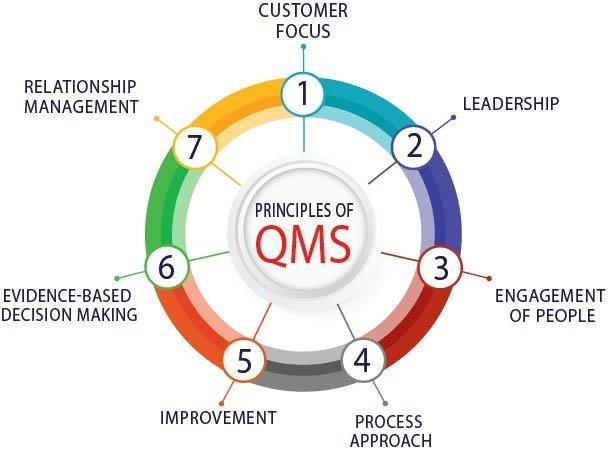
\includegraphics[width=.5\textwidth]{img/qms_iso9001.jpg}
%	\caption{Die sieben Grundsätze des QMS}
%\label{fig:qms_principles}
%\end{figure}

%\begin{figure}
%\includegraphics[scale=0.6]{} 
%\caption{}
%\end{figure}


\textcolor{red}{Reparaphrase!!}

\subsection{Warum digitale QMS?}
Das traditionelle QMS ist die Grundlage für ein digitales QMS, jedoch durch Redundanz charakterisiert. Digitale QMS arbeitet in die Gegenrichtung, da es darauf ausgerichtet ist, Redundanz zu vermeiden \cite{ibrahim2019digital}. Digitale QMS unterstützen den abteilungsübergreifenden Datenfluss in einer Organisation auf automatisierte Weise und verringern die Notwendigkeit manueller Übertragungen, die anfällig für menschliche Fehler und zeitaufwändig sind. Digitale QMS ersetzen papiergestützte QMS, da sie auf Echtzeit-Messungen und Feedback-Mechanismen beruhen, die eine zeitnahe Reaktion auf Ausfälle und Fehler ermöglichen. \cite{yeung2003empirical}


\section{Wesentliche Kriterien für die Auswahl eines QMS}

TODO

\subsubsection{Kriterium A: Industriebranche}

TODO



\subsubsection{Kriterium B}

TODO



\subsubsection{Kriterium C}

 TODO



\subsubsection{Kriterium D}

 TODO



\section{Fazit}

 TODO



\newpage
\phantomsection
\addcontentsline{toc}{section}{Literatur}
%\nocite{*}
\printbibliography
\end{document}
% ----------------------------------------------------------------------------
